\documentclass{article}

\usepackage{amsmath}
\usepackage{amsthm}
\usepackage{amsfonts}
\usepackage{framed}

%% Simple AMSthm environments, numbered together.
\newtheorem{lem}{Lemma}
\newtheorem{thm}[lem]{Theorem}
\newtheorem{conj}[lem]{Conjecture}

\theoremstyle{definition}
\newtheorem{defn}[lem]{Definition}

\begin{document}
The difficulty of getting the various analyses to work properly on a
piece of code is tightly coupled with the complexity of the underlying
control flow graph. Pathologies that underly implementations of flow
functions may not arise in straight-line programs but become painfully
obvious when branches are introduced. Our benchmarks are designed to
illustrate that our analyses are robust to non-trivial control flow
structures.

Broadly speaking, we have three types of benchmark. The first type is
straight-line programs, which introduce no branches in control
structure. They are the easiest to handle, and our analyses are
accordingly precise on them. Simple branching programs are the second
type, and they introduce conditional branches into fold, but do not
exhibit loops. They are slightly more challenging, but SSA makes them
much easier to handle. Our final type of benchmark is looping
programs. As their name suggests, they have loops, which makes
precision quite difficult. These benchmarks make sense because they
represent natural thresholds of program complexity, in terms of
language features.

\subsection{Constant Propagation}
\begin{center}
  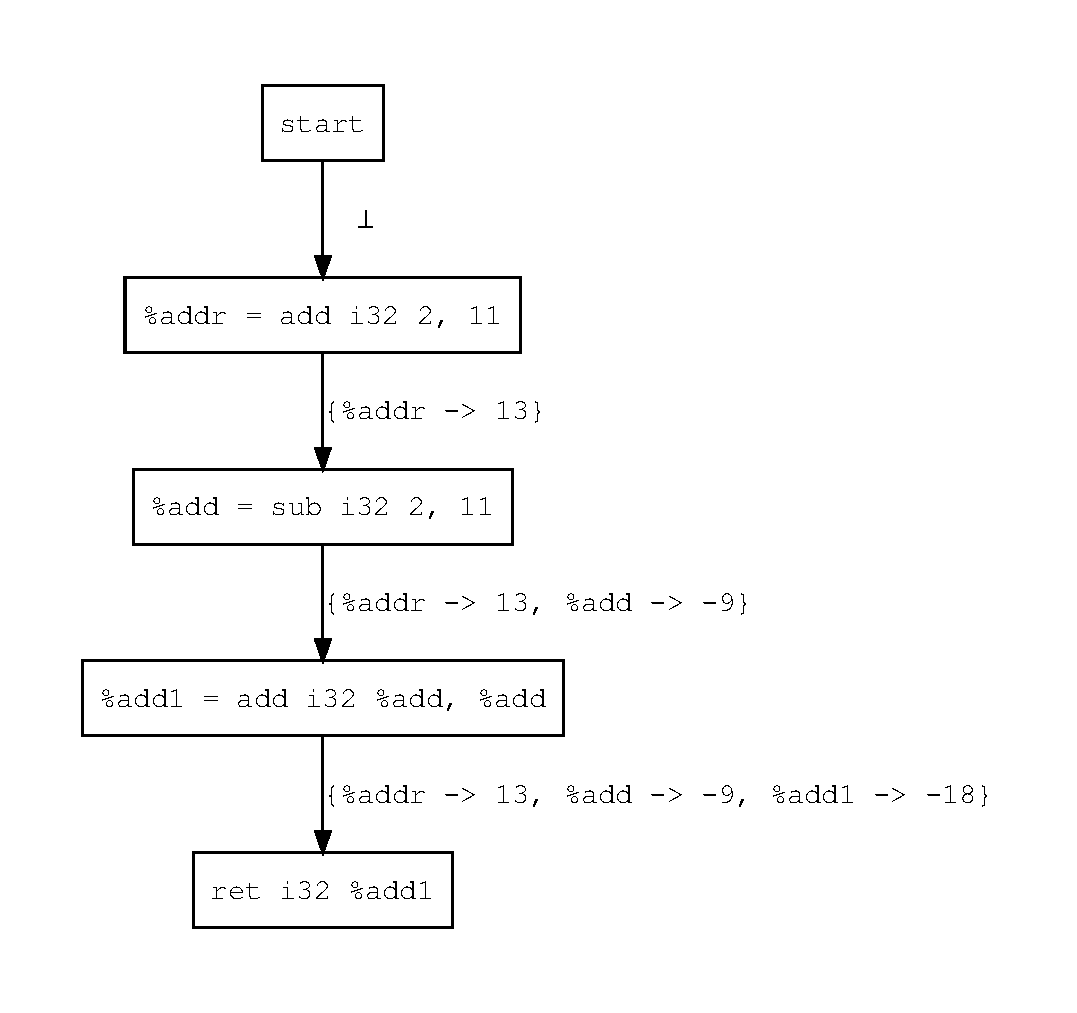
\includegraphics[scale=.4]{figures/cp/simple_add/simple_add.pdf}
  \captionof{figure}{Constant propagation analysis on a straight line program}
\end{center}

\begin{center}
  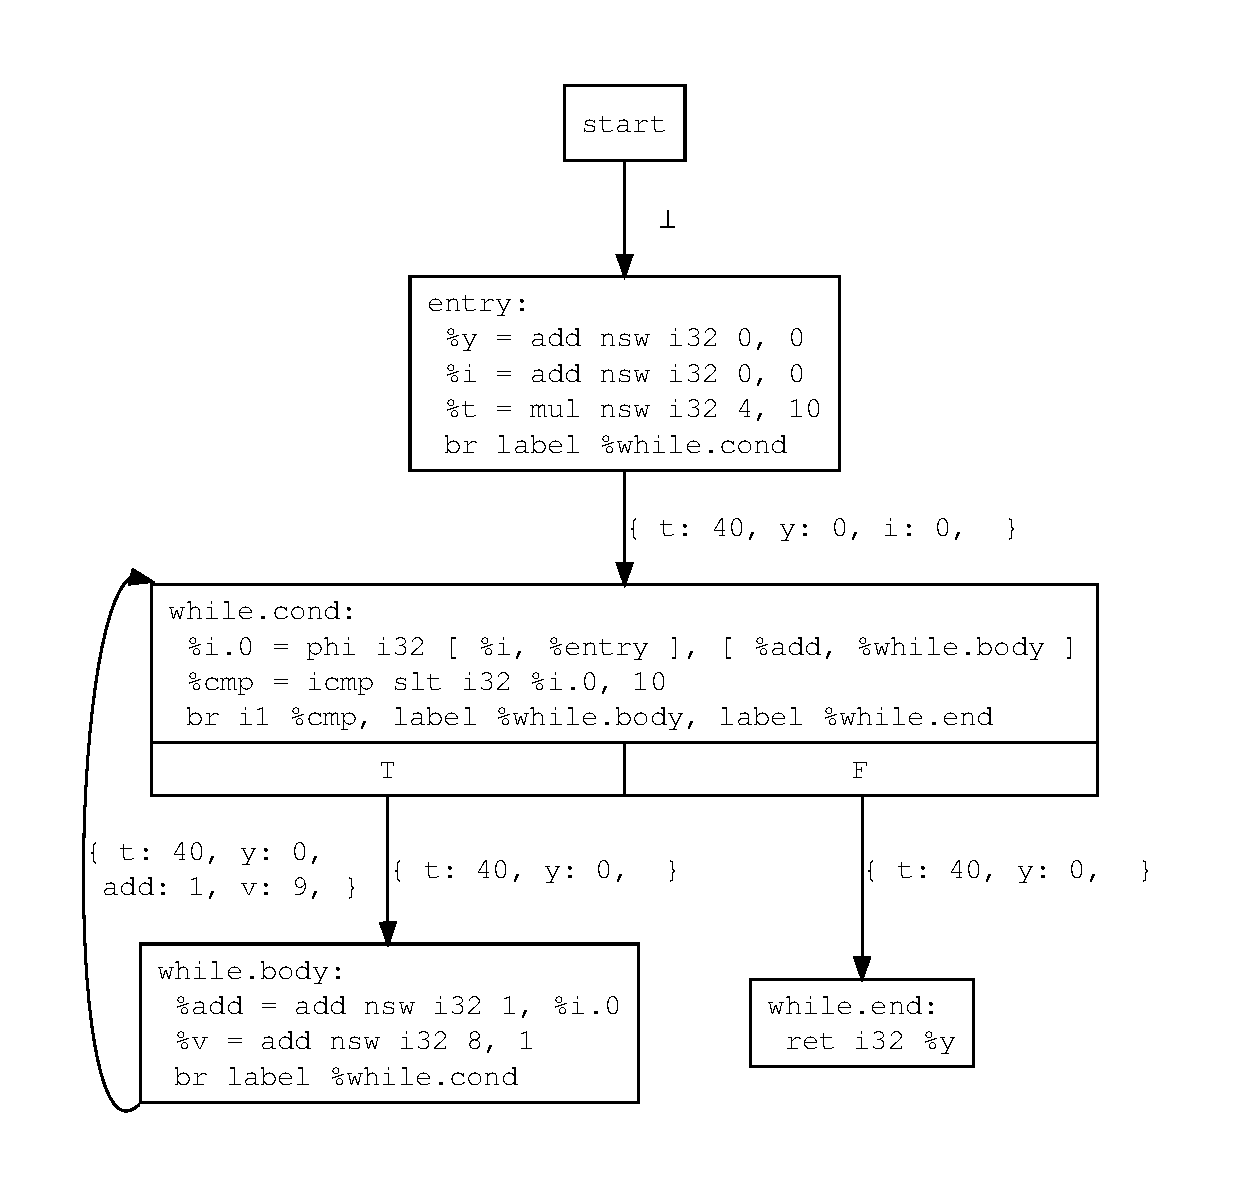
\includegraphics[scale=.4]{figures/cp/cp_loop/cp_loop.pdf}
  \captionof{figure}{Constant propagation analysis on a looping program}
\end{center}

Strangely, the looping test incorrectly believes that \texttt{add} is
the constant ``1'' for a single step. This is a problem with how the
merge is coded, but it seems to only affect the exit edges of the
bodies of loops and gets joined out later. For example, after the
relevent $\varphi$ function the analysis is correct again, but this is
not depicted in the figure. Please run the benchmark to examine the
output.

\subsection{Available Expressions}
\begin{center}
  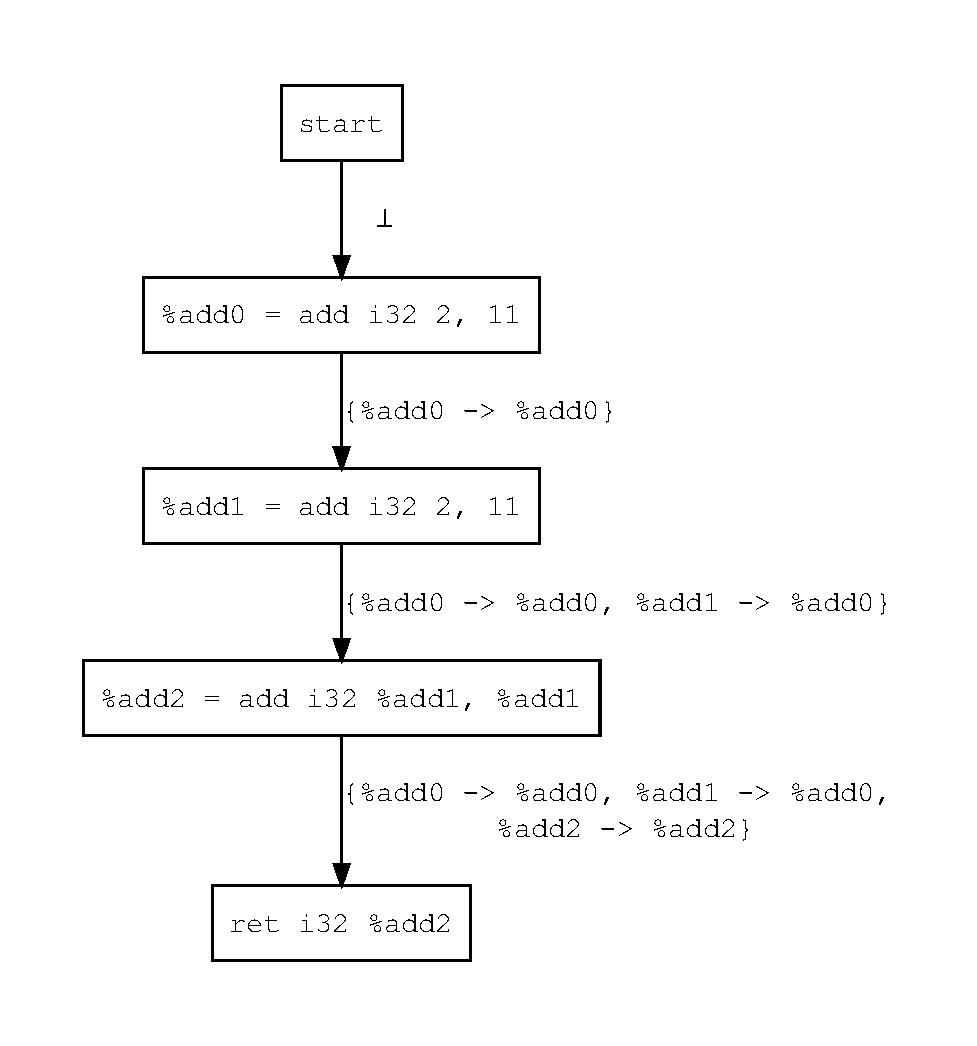
\includegraphics[scale=.4]{figures/cse/straight-line/can-do.pdf}
  \captionof{figure}{Available expression analysis of a straight-line program
    where CSE is possible}
\end{center}

\begin{center}
  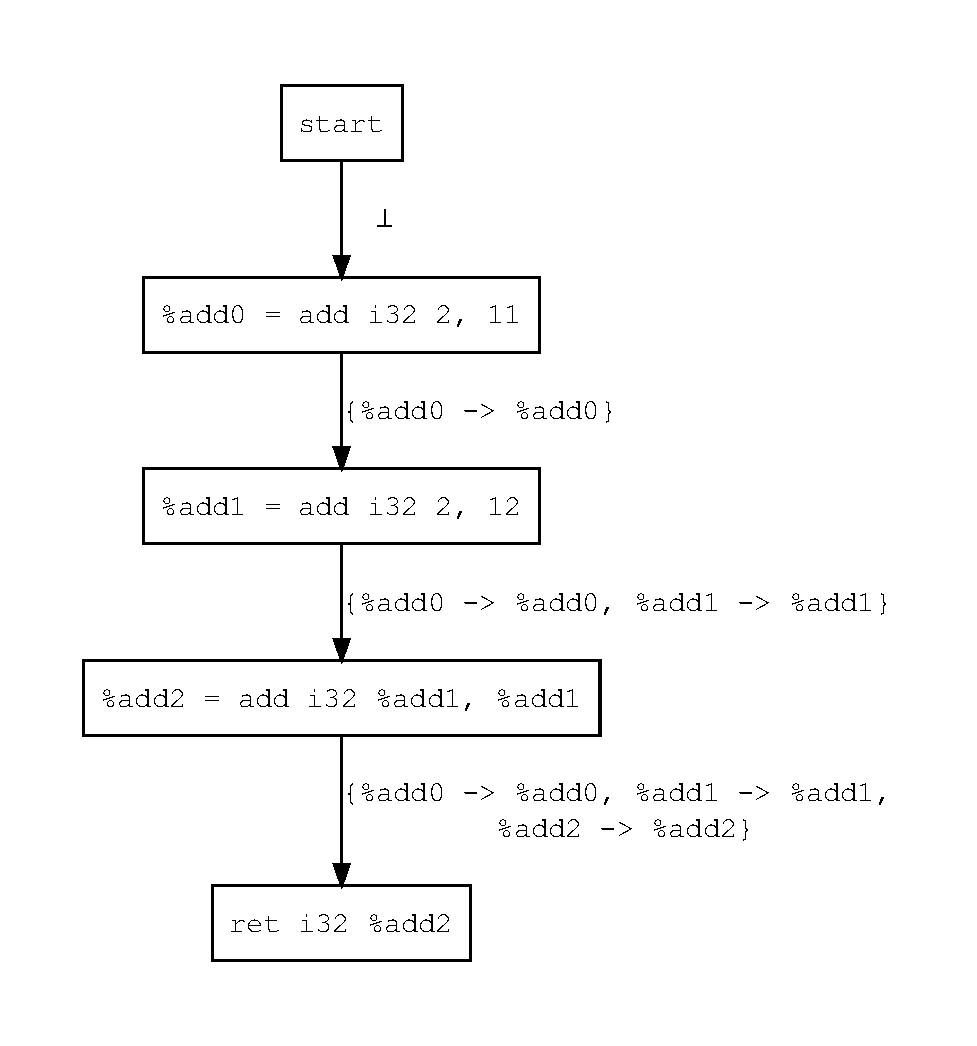
\includegraphics[scale=.4]{figures/cse/straight-line/no-do.pdf}
  \captionof{figure}{Available expression analysis of a straight-line program
    where CSE is not possible}
\end{center}

\begin{center}
  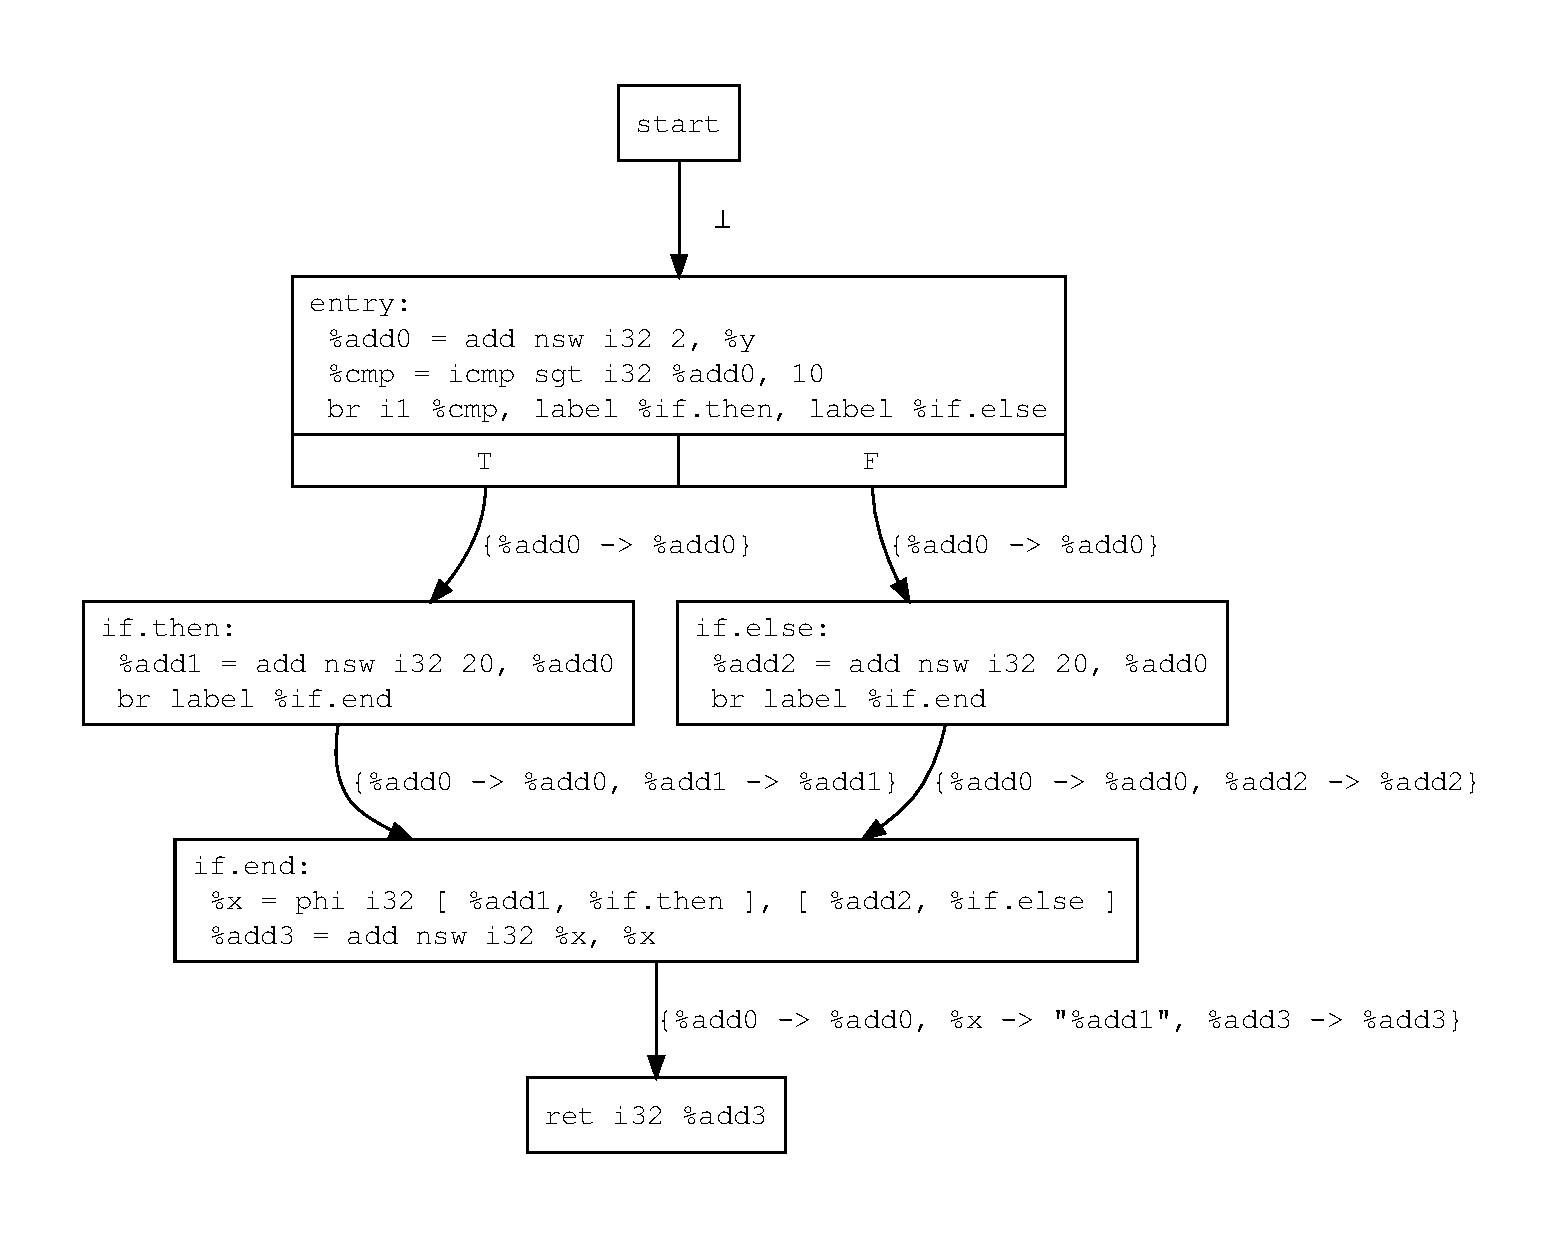
\includegraphics[scale=.4]{figures/cse/branch/can-do-cse.pdf}
  \captionof{figure}{Available expression analysis of a branching program
    where CSE is possible}
\end{center}

\begin{center}
  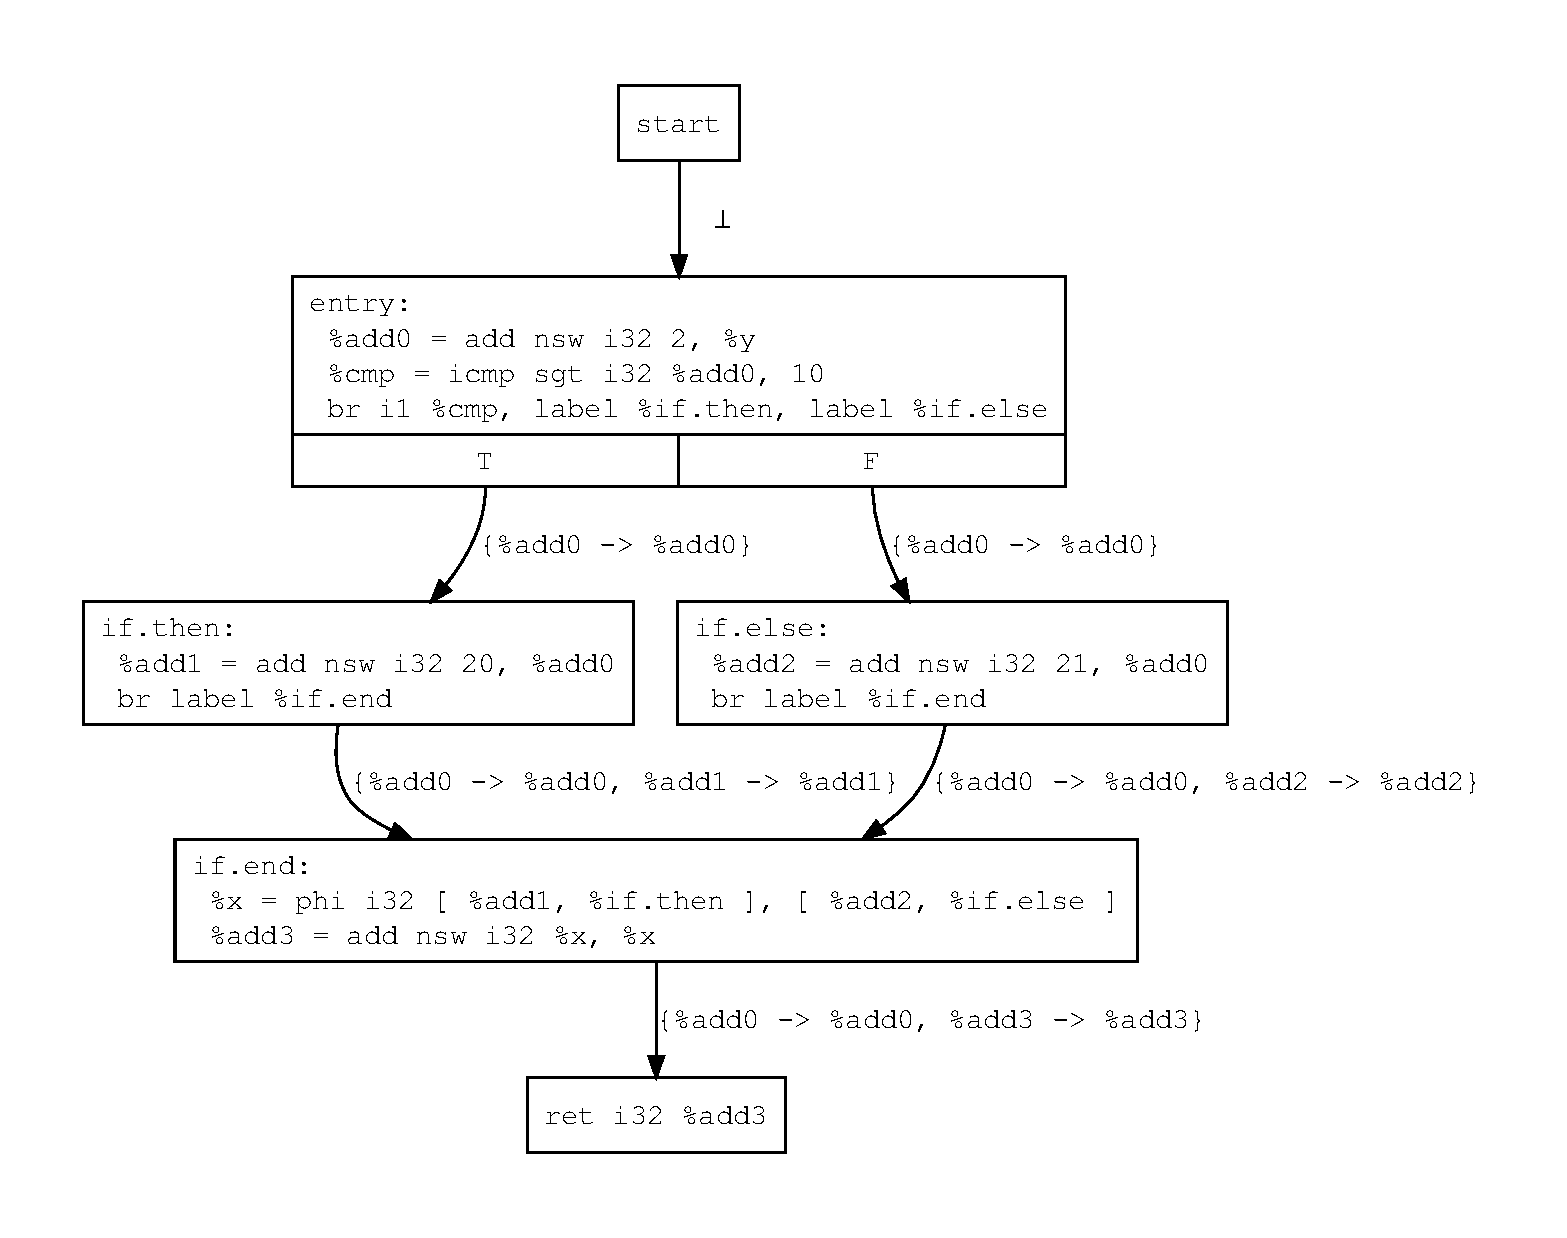
\includegraphics[scale=.4]{figures/cse/branch/no-do.pdf}
  \captionof{figure}{Available expression analysis of a branching program
    where CSE is not possible}
\end{center}

\begin{center}
  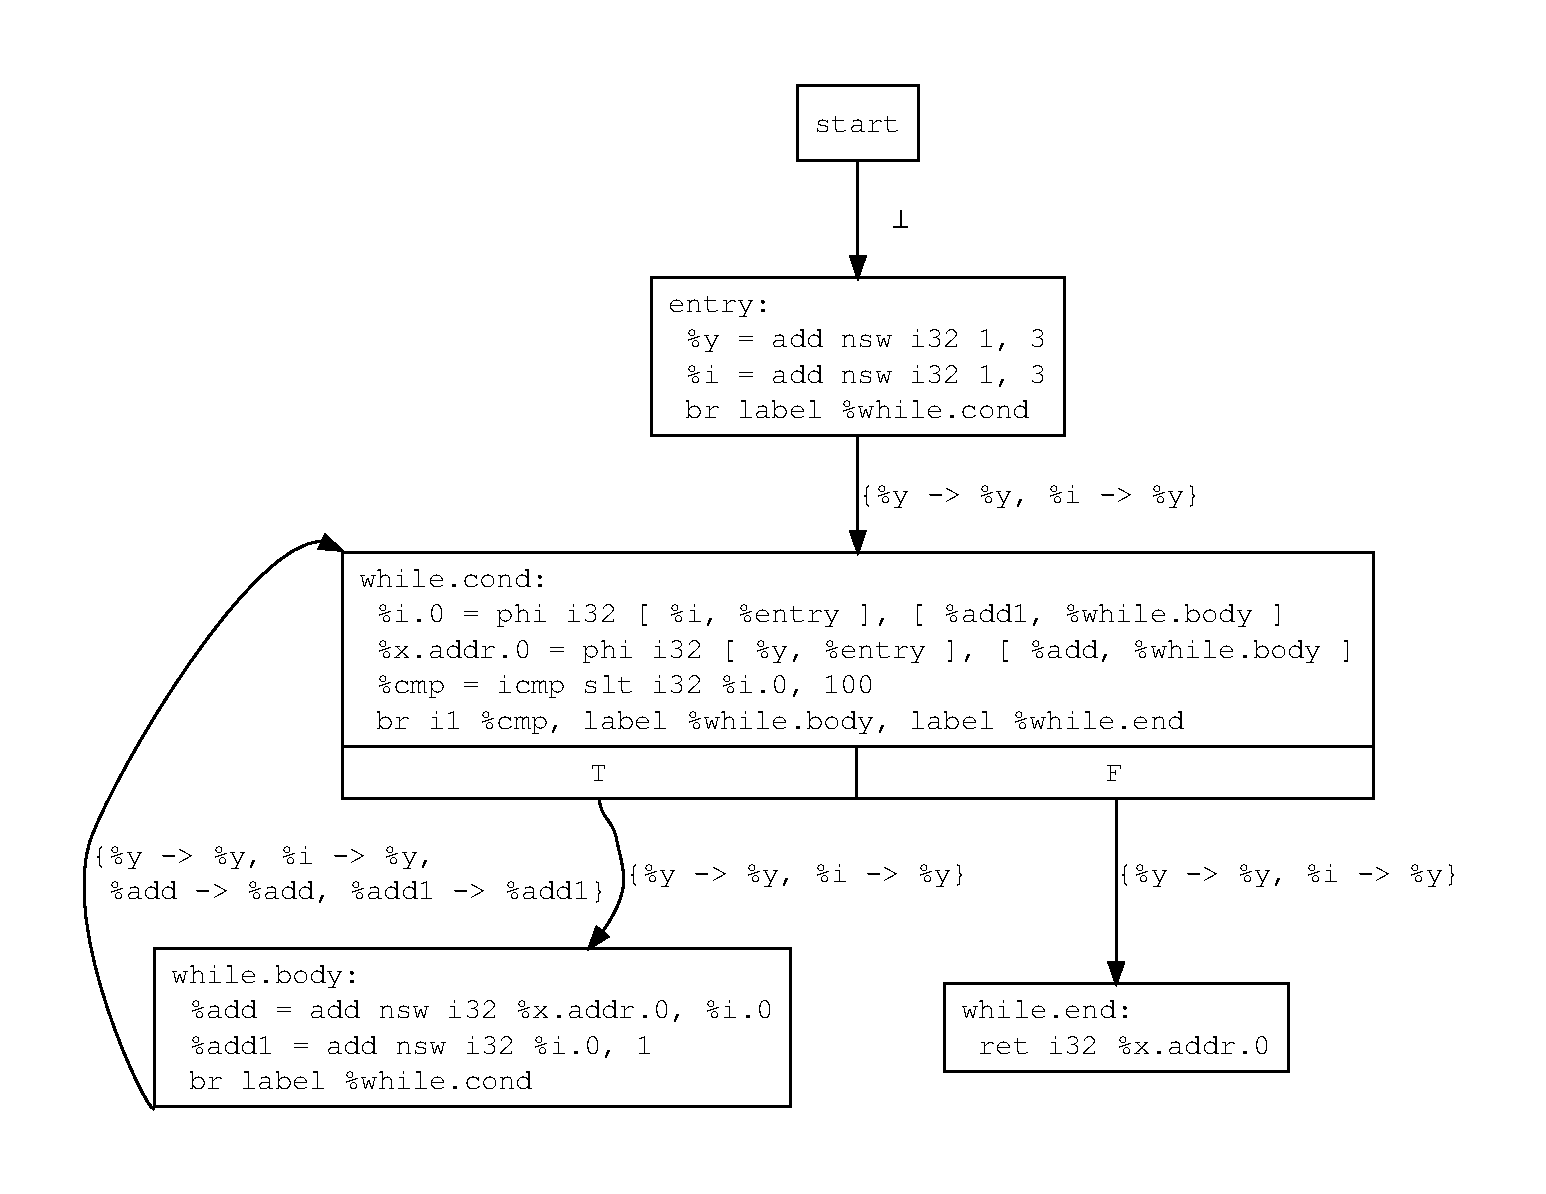
\includegraphics[scale=.4]{figures/cse/loop/loop-can-do-cse.pdf}
  \captionof{figure}{Available expression analysis of a looping program
    where CSE is possible}
\end{center}

\begin{center}
  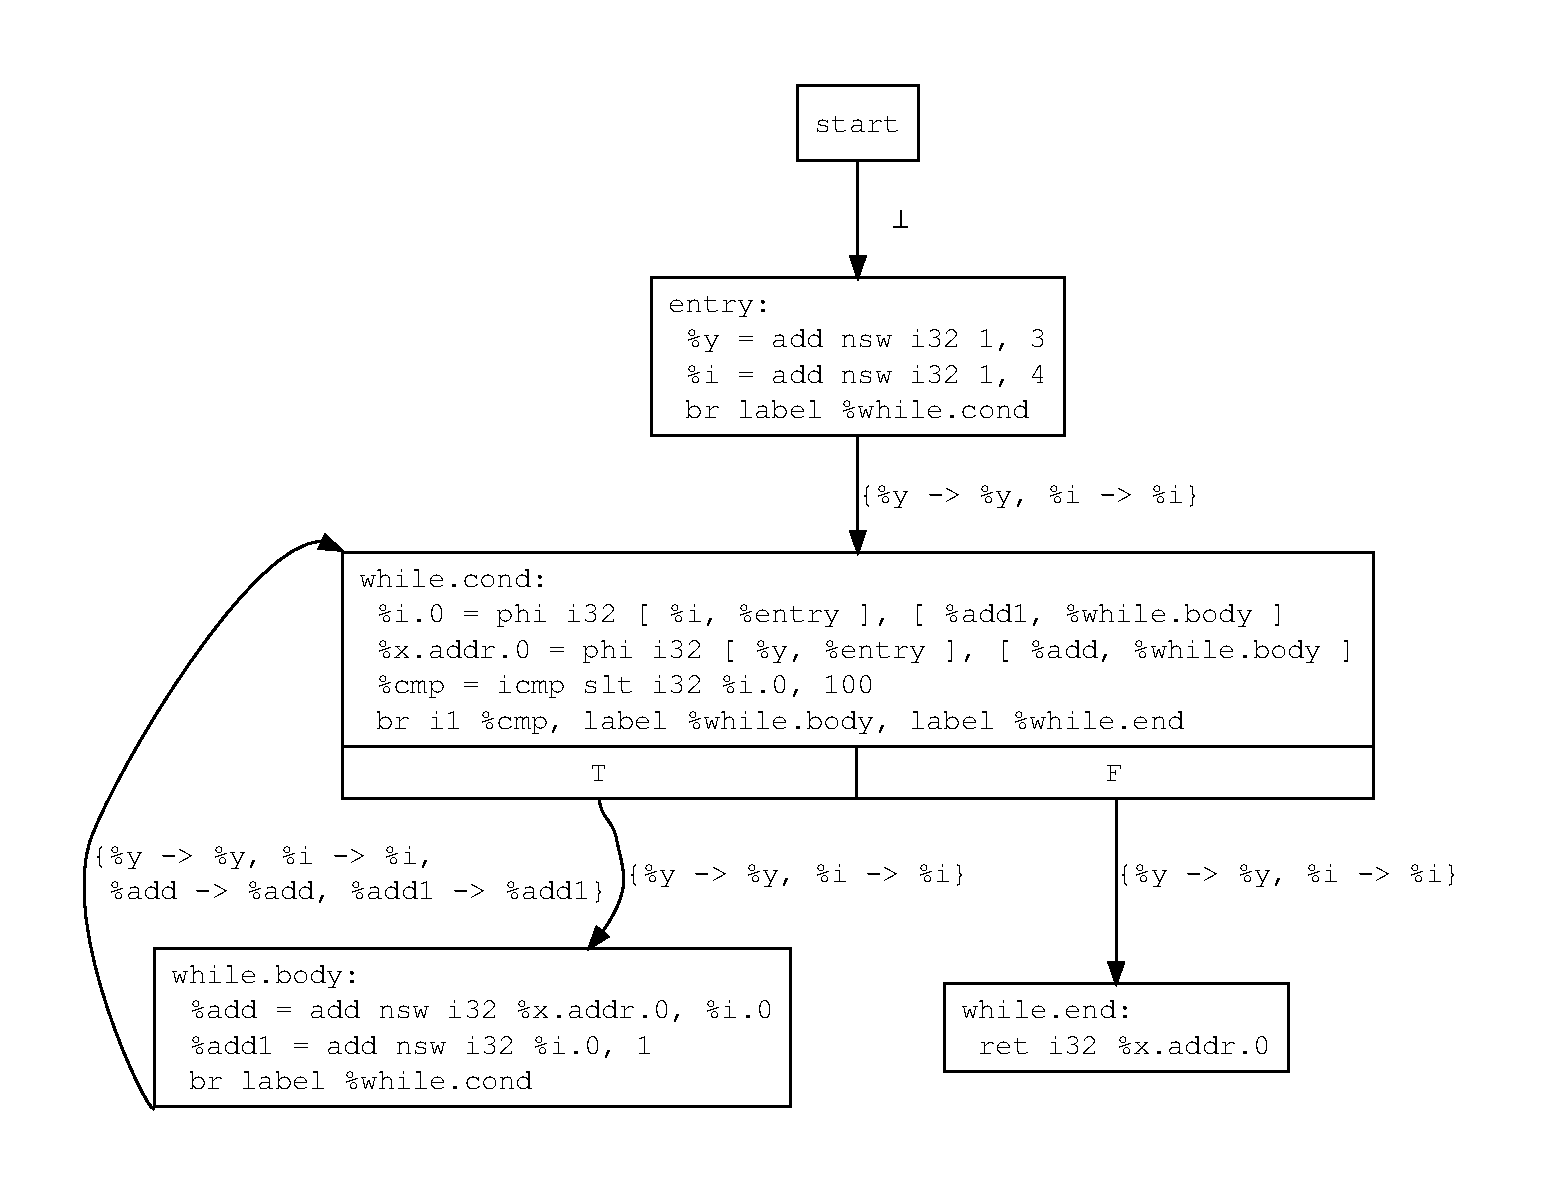
\includegraphics[scale=.4]{figures/cse/loop/loop-no-do-cse.pdf}
  \captionof{figure}{Available expression analysis of a looping program
    where CSE is not possible}
\end{center}

All tests passed.
\subsection{Range Analysis}
\begin{center}
  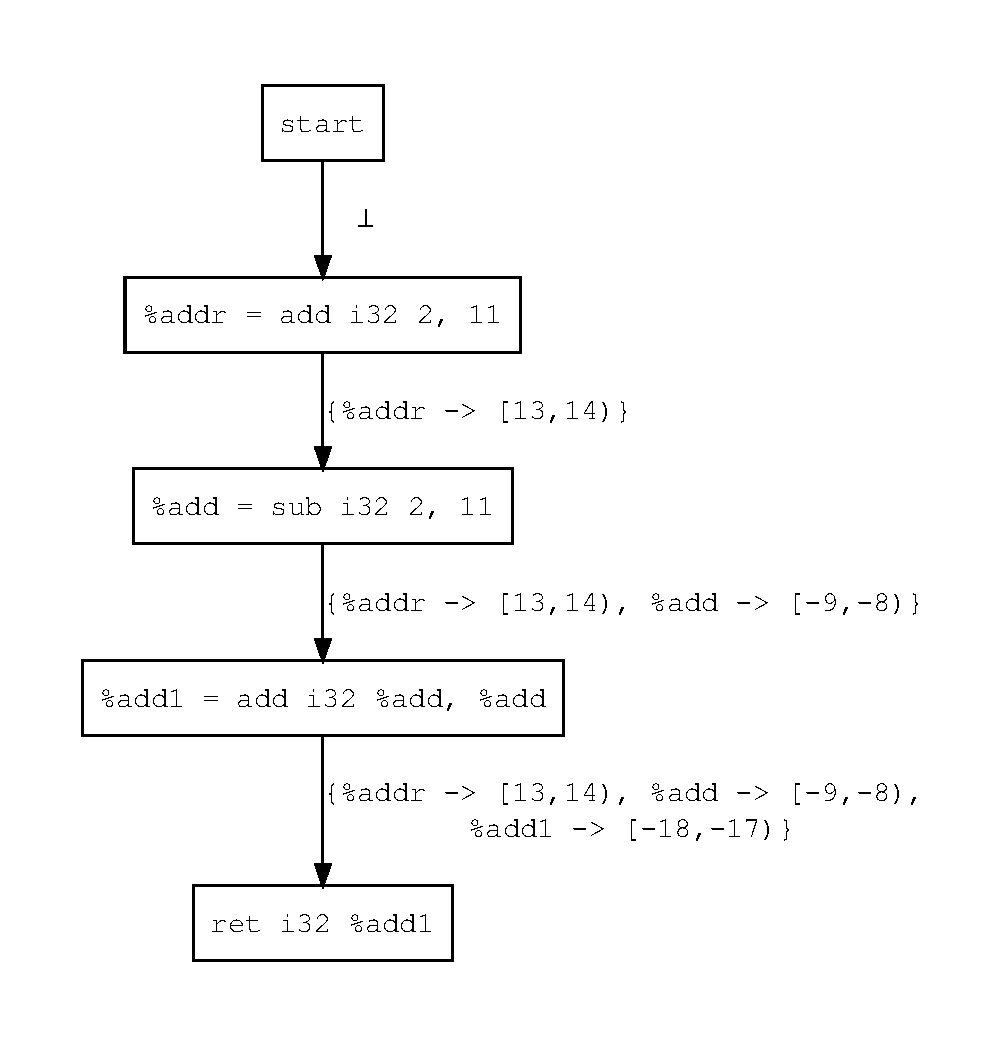
\includegraphics[scale=.4]{figures/ra/simple_add/simple_add.pdf}
  \captionof{figure}{Range analysis of a straight line program}
\end{center}
\begin{center}
  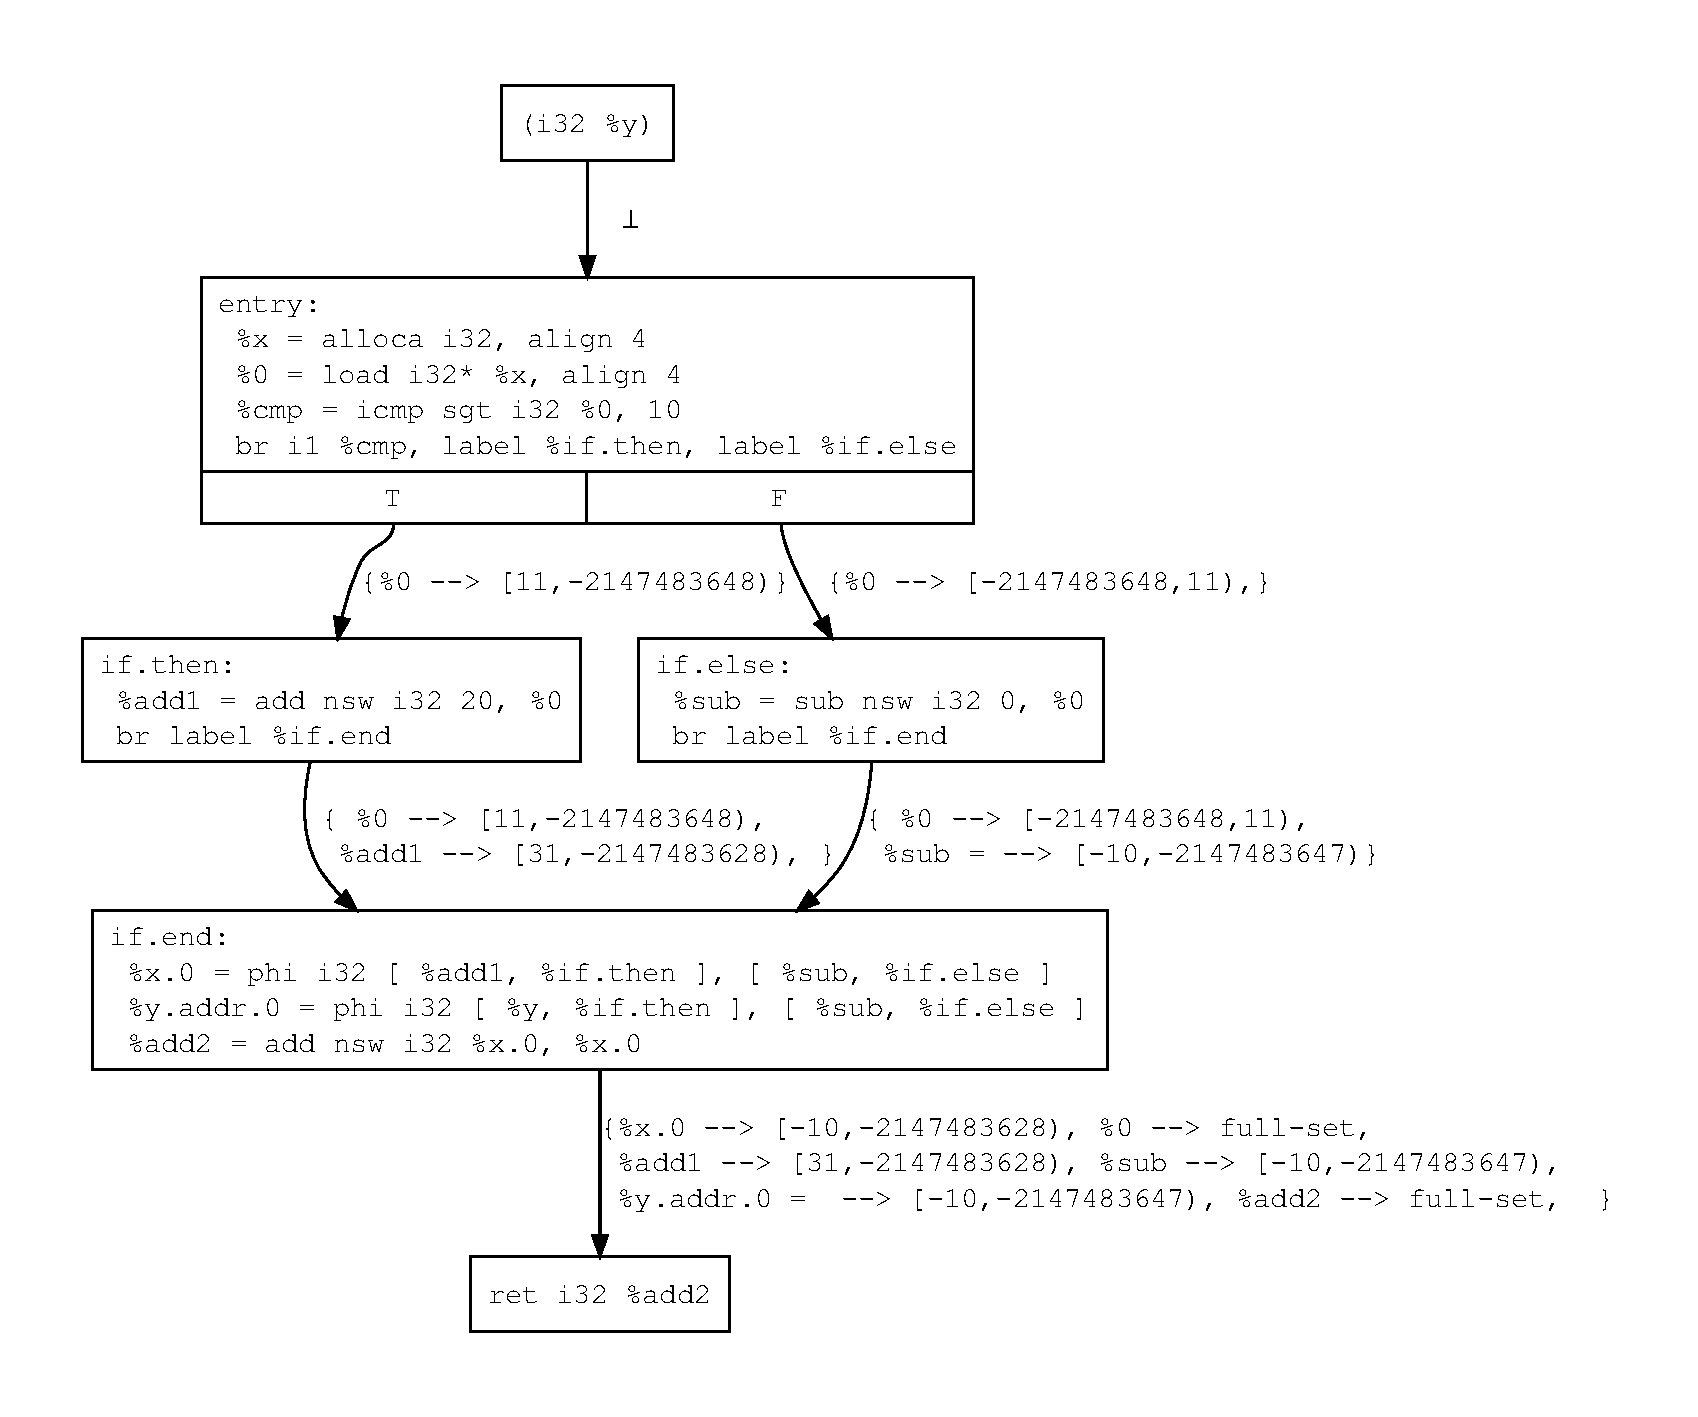
\includegraphics[scale=.4]{figures/ra/simple_branch/simple_branch.pdf}
  \captionof{figure}{Range analysis of a branching program}
\end{center}
\begin{center}
  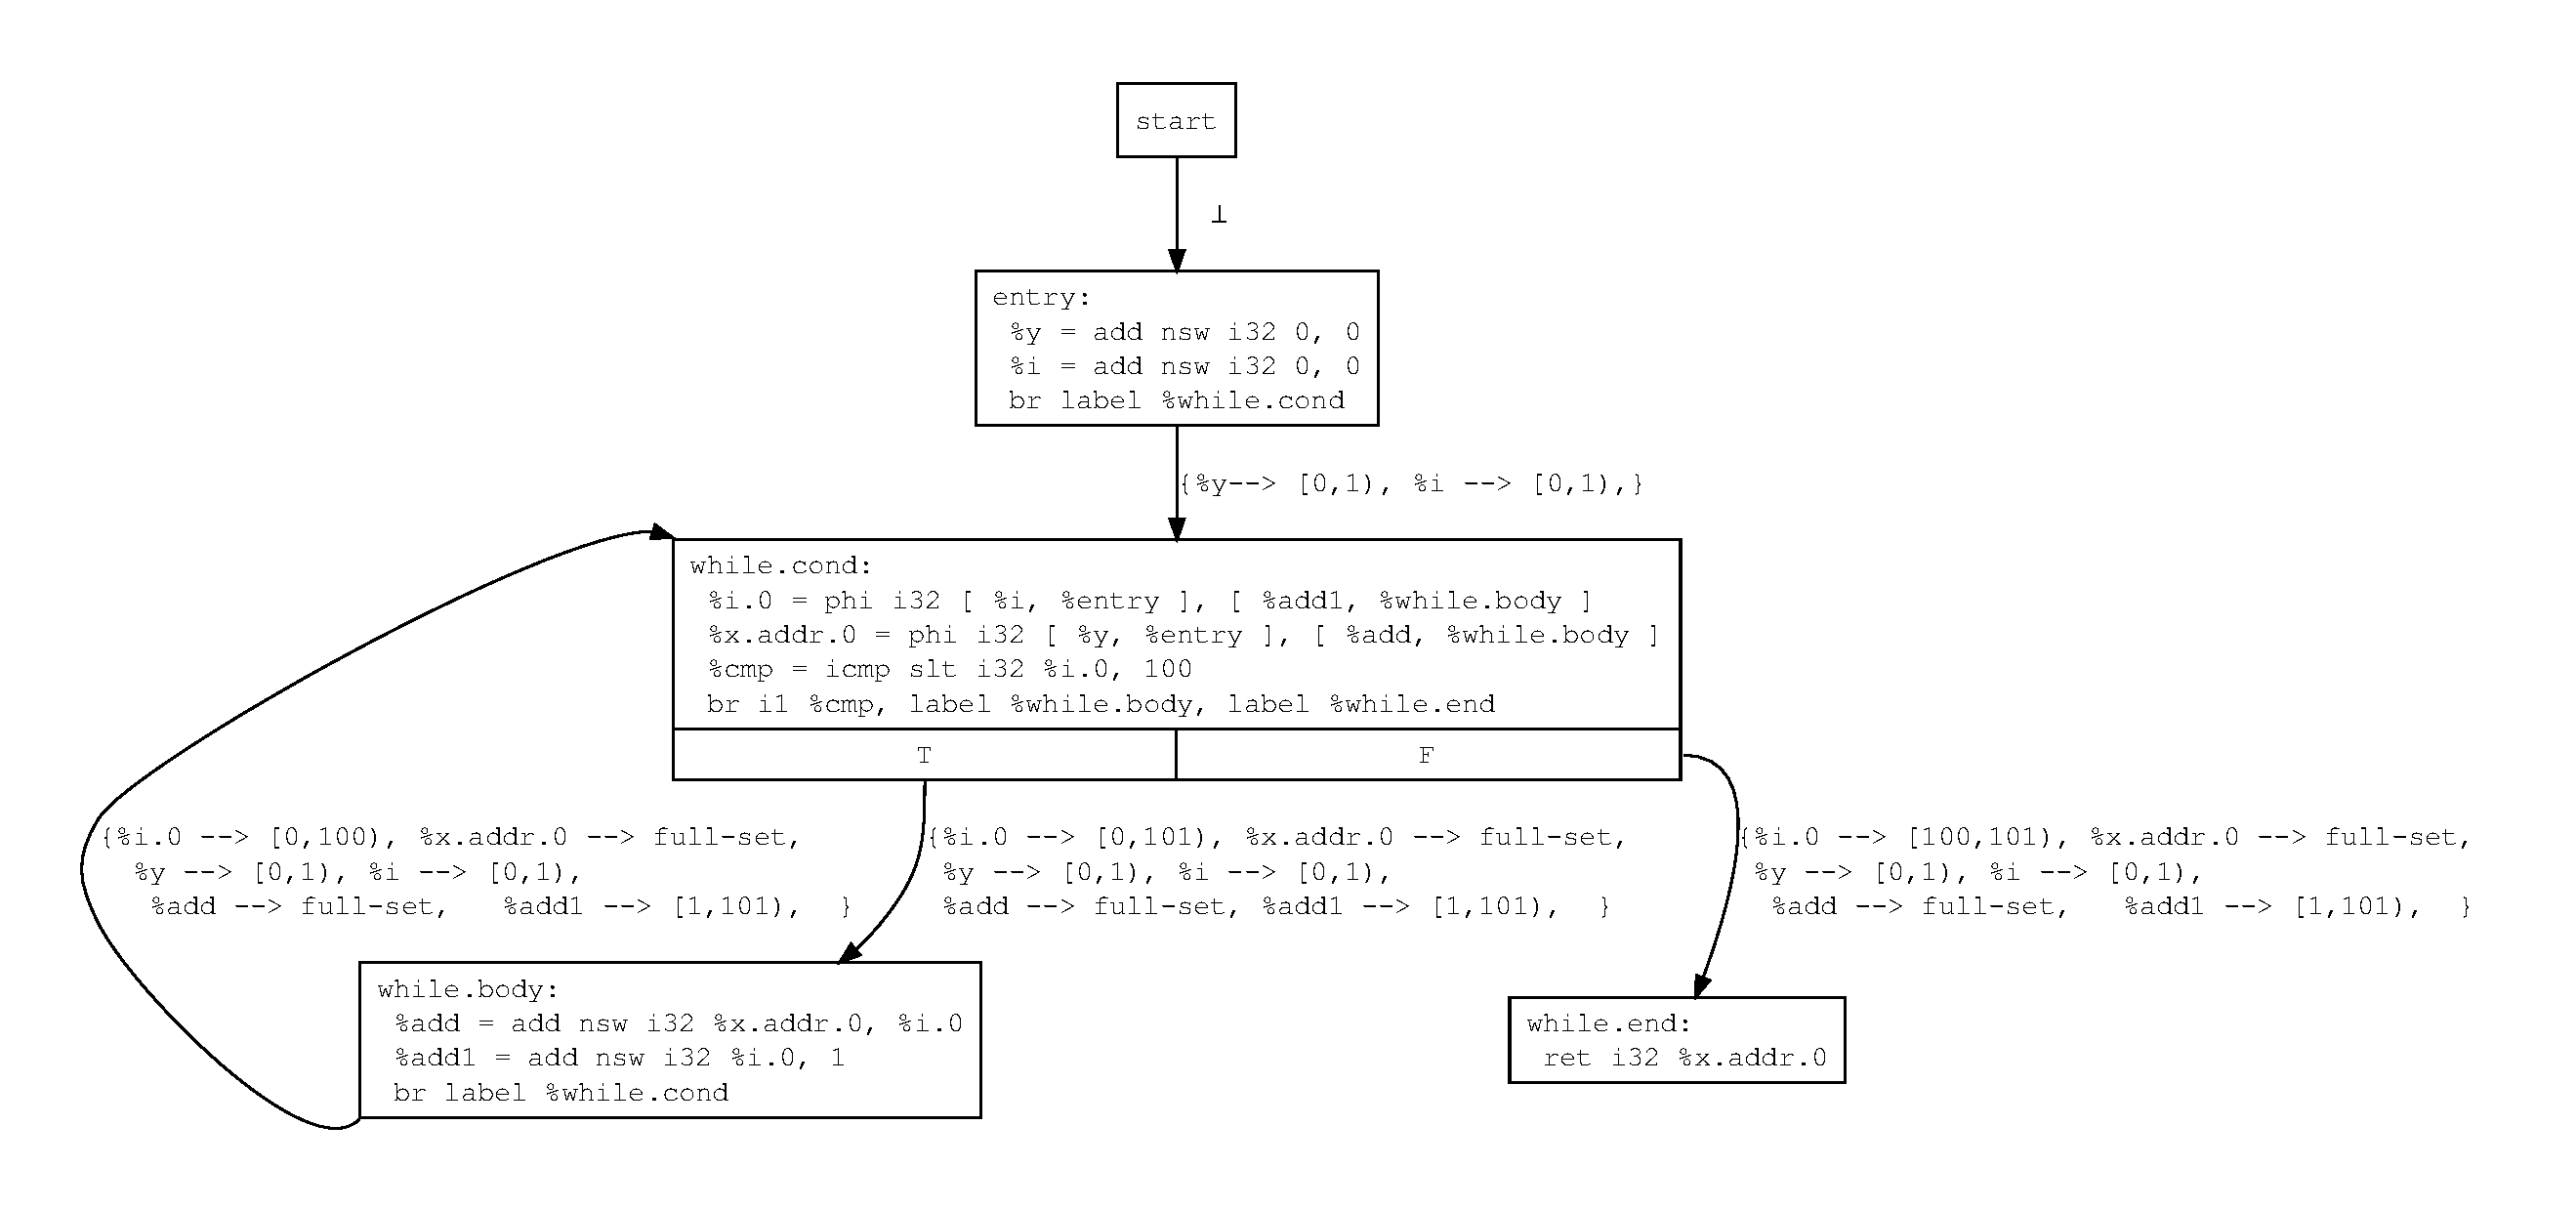
\includegraphics[scale=.4]{figures/ra/loop/loop.pdf}
  \captionof{figure}{Range analysis of a looping program}
\end{center}

All tests passed.
\subsection{Intra-Procedural Pointer Analysis}
See the file ``README.txt'' for how to run our tests, under the
Pointer Analysis heading. All tests were successful for this
analysis. We checked the analysis on straight line, branching, and
looping programs, as for the analyses above.
\subsection{Range Checking}

As per the assignment, we also implemented a range checking pass to
make sure that array accesses remain inbound and raise warnings
otherwise. This was fairly straightforward once the range analysis
work was completed. To do this part, we simply ran our range analysis
on the incoming function, then we scanned through the instructions for
a getelementptr instruction. We then look at the lattice point at this
instruction, query the index range, and raise a warning if it has a
range that potentially falls outside of the range of the array.

These warnings operated correctly in our tests. To run them, see the
file ``README.txt''.
\end{document}

